\documentclass{standalone}

\usepackage{tikz}
\usepackage{ctex}

\begin{document}
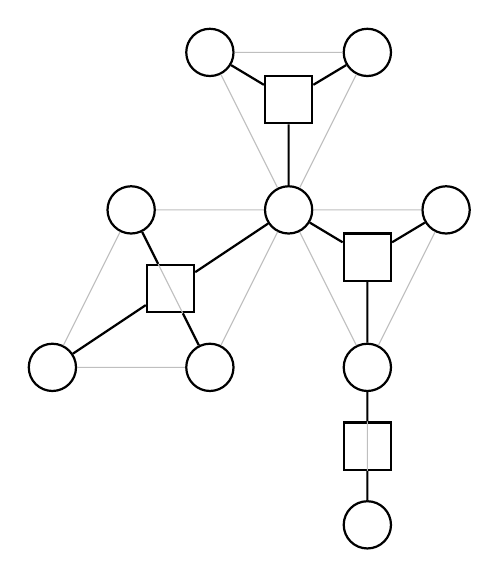
\begin{tikzpicture}[x=20mm,y=20mm]

\begin{scope}[every node/.style={draw,minimum size=6mm},circle,thick]
    \node (GA) at (-0.5,1){};
    \node (GB) at (0.5,1) {};
    \node (GC) at (0,0) {};
    \node (GD) at (-1,0) {};
    \node (GE) at (-0.5,-1) {};
    \node (GF) at (-1.5,-1) {};
    \node (GG) at (1,0) {};
    \node (GH) at (0.5,-1) {};
    \node (GI) at (0.5,-2) {};

\begin{scope}[rectangle]
    \node (FA) at (0,0.7) {};
    \node (FB) at (-0.75,-0.5) {};
    \node (FC) at (0.5,-0.3) {};
    \node (FD) at (0.5,-1.5) {};
\end{scope}
\end{scope}

\draw[color=lightgray]
    (GA) -- (GB) -- (GC) -- (GA)
    (GC) -- (GD)
    (GC) -- (GE)
    (GD) -- (GE) -- (GF) -- (GD)
    (GC) -- (GG) -- (GH) -- (GC)
    (GH) -- (GI);

\draw[thick]
    (GA) -- (FA)
    (GB) -- (FA)
    (FA) -- (GC)
    (GC) -- (FB)
    (GC) -- (FC)
    (FB) -- (GD)
    (FB) -- (GE)
    (FB) -- (GF)
    (FC) -- (GG)
    (FC) -- (GH)
    (GH) -- (FD)
    (FD) -- (GI);


\end{tikzpicture}
\end{document}
